%05/02 - Raúl Guantes
\chapter{Sistemas dinámicos no lineales}
\section{Crecimiento logístico}
El crecimiento de las poblaciones biológicas está limitado por la disponibilidad de recursos. Para modelar este fenómeno, se introduce un nuevo parámetro $k$, que representa la capacidad de carga del entorno, es decir, la cantidad máxima de individuos que el entorno puede sostener (la cantidad de recursos disponibles para toda la población). Además, se considera:
\begin{itemize}
\item $r$: la \textbf{tasa de crecimiento} de una población (positiva)
\item $N(t)$: el número de células en el tiempo $t$
\end{itemize}
La dinámica de la población se describe mediante una ecuación diferencial que depende de $N$, $r$ y $k$:
$$\frac{dN}{dt} = f(N; r, k)$$

\subsection{Ecuación de crecimiento logístico}
Si los recursos son ilimitados, la población crece exponencialmente:
$$\frac{dN}{dt} = rN$$

Sin embargo, cuando los recursos son limitados, el crecimiento se ve afectado por la disponibilidad de recursos. Si la población supera la capacidad de carga ($N > k$), la población disminuye debido a la falta de recursos. Por el contrario, si la población es pequeña ($N < k$), hay suficientes recursos para que la población crezca. Esto se modela mediante la \textbf{ecuación de crecimiento logístico}:
$$\frac{dN}{dt} = rN(1-\frac{N}{k})$$
Esta ecuación es \textbf{no lineal} debido al término $N^2$. Se puede obtener la derivada para ver si la población crece (derivada positiva) o disminuye (derivada negativa).

\subsection{Solución de la ecuación logística}
La solución analítica de la ecuación logística es:
$$N(t) = \frac{N(0) k}{N(0) + (k - N(0))e^{-rt}}$$
Cuando $t \rightarrow \infty$, la población tiende a la capacidad de carga $k$, alcanzando un \textbf{estado de equilibrio}:
$N(t) \rightarrow k$

\subsection{Puntos de equilibrio y estabilidad}
En un sistema dinámico, los \textbf{puntos de equilibrio} son aquellos en los que la derivada temporal es cero ($dN/dt = 0$). Para la ecuación logística, los puntos de equilibrio son:
$$0 = r N (1 - \frac{N}{K}) \begin{cases} 
N^1_{eq} = K \rightarrow \text{Estable} \\
N^2_{eq} = 0 \rightarrow \text{Inestable}
\end{cases}
$$

\begin{itemize}
\item $N_{eq} = k$ es un punto de equilibrio estable, ya que la población tiende a $k$ a largo plazo.
\item $N_{eq} = 0$ es un punto de equilibrio inestable, ya que cualquier pequeña perturbación hará que la población crezca hacia $k$.
\end{itemize}

\begin{figure}[h]
\centering
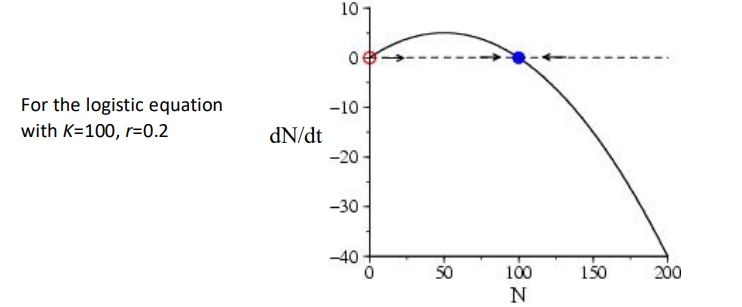
\includegraphics[width = 0.9\textwidth]{figs/estabilidad-dinamica.png}
\end{figure}

\subsection{Análisis de estabilidad}
Para entender el comportamiento a largo plazo de un sistema dinámico, es necesario calcular los puntos de equilibrio y determinar su estabilidad. 
Un sistema biológico de verdad, al medir a tiempos largos, siempre va a estar en un estado de equilibrio estable, al ser robustos a fluctuaciones. La estabilidad se puede deducir sin resolver la ecuación diferencial mediante dos formas: la forma gráfica y la forma matemática. 

\subsubsection{Método gráfico: Plano de fases}
En sistemas con una sola variable, se utiliza el plano de fases, donde:
\begin{itemize}
\item El eje x representa la variable $N$.
\item El eje y representa la derivada $dN/dt$
\end{itemize}
Para la ecuación logística:
$$\frac{dN}{dt} = f(N) = rN - \frac{rN^2}{K}$$ 
Esta función es una parábola invertida con puntos de corte en $N = 0$ y $N = k$. El máximo de la parábola se encuentra en:
$$\frac{df}{dN} = 0 \rightarrow r - \frac{2rN}{k} = 0 \rightarrow N = \frac{k}{2}$$

El punto $N = k$ es \textbf{estable} porque, a su izquierda, $dN/dt > 0$ (la población crece), y a su derecha, $dN/dt < 0$ (la población decrece).

\subsubsection{Método matemático: Linealización}
Este método es más general y puede aplicarse a sistemas con múltiples variables. Consiste en linealizar la función $f(N)$ alrededor de un punto de equilibrio $N_{eq}$ utilizando una \textbf{aproximación de Taylor}.
\begin{enumerate}
\item \textbf{Perturbación alrededor del equilibrio}
$$N = N_{eq} + \Delta N$$

\item \textbf{Derivada temporal}
$$\frac{dN}{dt} = \frac{d(N_{eq} + \Delta N)}{dt} = f(N_{eq} + \Delta N)$$

\item \textbf{Aproximación de Taylor} $f(N) \approx a + bN + cN^2 + dN^3 + \ldots$
$$f(N_{eq} + \Delta N) \approx f(N_{eq}) + \frac{df(N_{eq})}{dN} \Delta N$$
Como $f(N_{eq}) = 0$ (punto de equilibrio), se simplifica a:
$$\frac{d \Delta N}{dt} \approx f'(N_{eq}) \Delta N$$

\item \textbf{Solución de la ecuación linealizada}
$$\Delta N(t) = \Delta N(0) \cdot e^{f'(N_{eq})t}$$
\begin{itemize}
\item Si $f'(N_{eq}) > 0$, el punto de equilibrio es \textbf{inestable}, ya que la perturbación crece con el tiempo.
\item Si $f'(N_{eq}) < 0$, el punto de equilibrio es \textbf{estable}, ya que la perturbación decrece con el tiempo.
\item Si $f'(N_{eq}) = 0$, entonces se necesitan incluir términos de mayor orden de la serie de Taylor. 
\end{itemize}
\end{enumerate}

%13/02 - Raúl Guantes
\section{No linealidades superiores: biestabilidad y efecto Allee}
Cuando las células cooperan, el crecimiento de la población depende de su tamaño. Existe un \textbf{umbral crítico} $N*$, por debajo del cual la población se extingue. Esto se conoce como el \textbf{efecto Allee}.

Para que la población crezca, no solo es necesario que haya recursos disponibles, sino que también debe haber un tamaño mínimo de población para que la cooperación sea efectiva. Si $N < N*$, no hay cooperación y la población disminuye (la derivada es negativa). Si $N > N*$, la cooperación es efectiva y la población crece (la derivada es positiva).

La dinámica se modela con la siguiente ecuación diferencial:
$$\frac{dN}{dt} = rN (1 - \frac{N}{k}) (\frac{N}{N*} - 1)$$

\subsection{Puntos de equilibrio y estabilidad}
Los puntos de equilibrio se calculan igualando la derivada a cero:
$$\frac{dN}{dt} = 0 \rightarrow rN(1 - \frac{N}{k})(\frac{N}{N*} - 1) = 0$$

Los puntos de equilibrio son:
\begin{itemize}
\item $N^1_{eq} = 0$: Estable (la población se extingue).
\item $N^2_{eq} = N*$: Inestable (umbral crítico).
\item $N^3_{eq} = K$: Estable (capacidad de carga).
\end{itemize}

\begin{figure}[h]
\centering
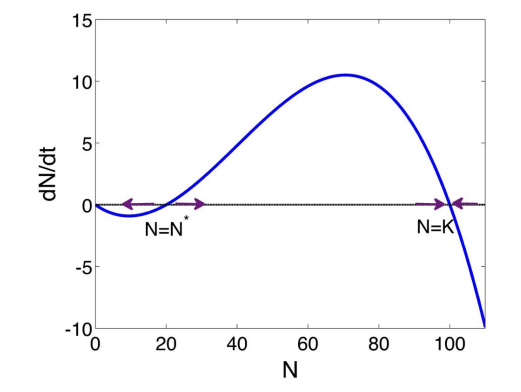
\includegraphics[width = 0.7\textwidth]{figs/bistability-graph.png}
\end{figure}

La coexistencia de dos estados de equilibrio estables se denomina \textbf{biestabilidad} (o multiestabilidad si hay más de dos). El estado final de la población depende de las condiciones iniciales:
\begin{itemize}
\item Si $N(0) > N*$, la población tiende a $k$.
\item Si $N(0) < N*$, la población tiende a 0.
\end{itemize}

El punto de equilibrio inestable $N*$ actúa como un \textbf{separador} entre los dos estados estables.

\begin{figure}[h]
\centering
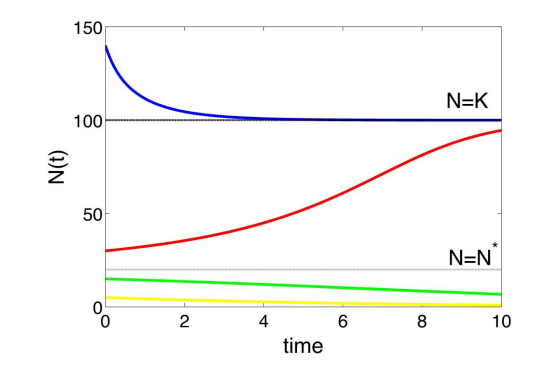
\includegraphics[width = 0.7\textwidth]{figs/bistability.png}
\end{figure}

\subsection{Bifurcaciones}
Al variar el parámetro $N*$, pueden aparecer o desaparecer puntos de equilibrio, o cambiar su estabilidad. Esto se conoce como \textbf{bifurcación}. Un ejemplo es cuando $N* = k$, donde ocurre un cambio crítico en la estabilidad.

\begin{figure}[h]
\centering
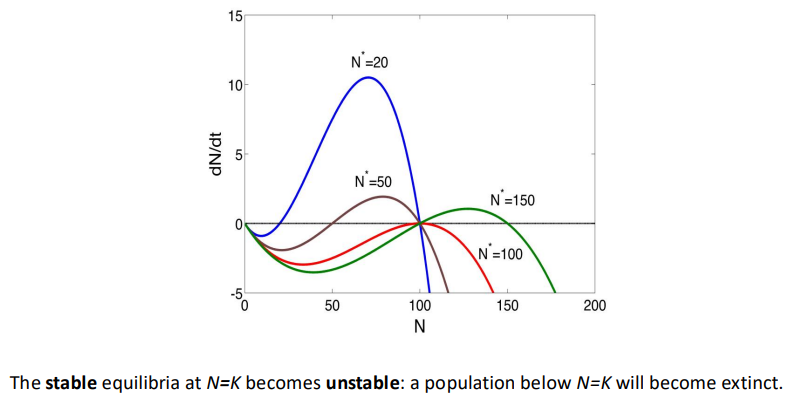
\includegraphics[width = 0.7\textwidth]{figs/bistability-bifurcations.png}
\caption{\textbf{Bifurcaciones al variar N*.} K está fijado, y N* se va aumentando progresivamente, independientemente de su sentido biológico. La línea roja representa un valor N*=k, y a partir de ahí cambia la estabilidad; ese es el punto de bifurcación, y en ese punto la derivada es 0 y la linealización falla.}
\end{figure}

Un \textbf{diagrama de bifurcación} muestra los puntos de equilibrio en función de un parámetro (por ejemplo, $N*$). Las líneas continuas representan estados estables, y las discontinuas, estados inestables.

\begin{figure}[h]
\centering
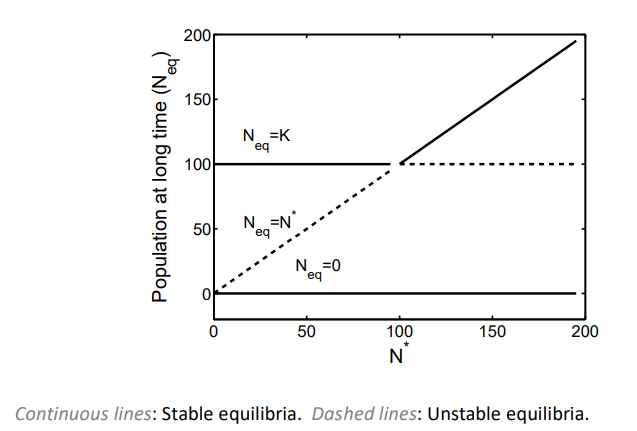
\includegraphics[width = 0.7\textwidth]{figs/bifurcation-diagram.png}
\caption{Diagrama de bifurcación. Las líneas continuas representan los estados estables, y las líneas discontinuas los estados inestables. Se representan los tres puntos de equilibrio 0, k y N*. El punto (0,0) se considera punto de bifurcación, ya que es donde cambian de estabilidad los puntos de equilibrio k y N*.}
\end{figure}

\subsection{Muerte por macrófagos: biestabilidad con histéresis}
Consideremos una población de células cancerígenas $N$ que es atacada por macrófagos (células inmunes). La dinámica se describe como:
$$\frac{dN}{dt} = rN(1 - \frac{N}{K}) - p(N)$$
donde $p(N) = N^2/(1 + N^2)$ modela el efecto de los macrófagos.

Los puntos de equilibrio se obtienen resolviendo:
$$rN(1 - \frac{N}{K}) = \frac{N^2}{1 + N^2}$$
El primer punto de equilibrio es en 0. Para el resto, se pueden solapar las rectas $r(1 - \frac{N}{k})$ sobre la función $\frac{N}{1 + N^2}$ y ver los puntos de corte. Dependiendo de r, puede haber de 1 a 4 puntos de corte. 

\begin{figure}[h]
\centering
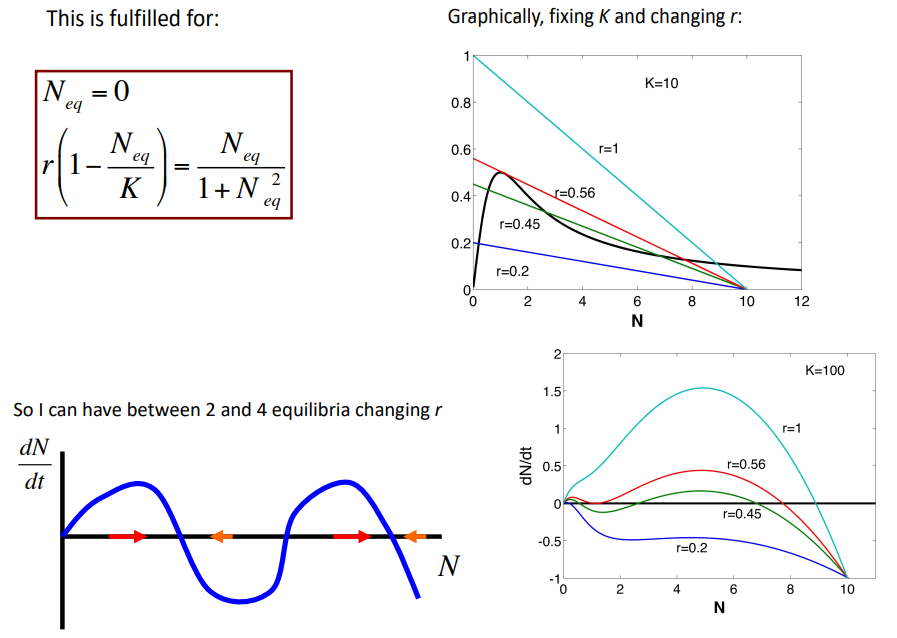
\includegraphics[width = 0.7\textwidth]{figs/biestabilidad-histeresis.png}
\caption{El estado 0 es trivial, es inestable. Si hay varios puntos de equilibrio estables, entre ellos siempre debe haber un estado inestable.}
\end{figure}

Al variar $r$, pueden aparecer múltiples puntos de equilibrio. El sistema muestra \textbf{histéresis}: el comportamiento no es simétrico al aumentar o disminuir $r$.

\newpage

Si dibujamos este diagrama de bifurcación, hay un punto en el cuál se diferencian los puntos estable e inestable. Hay dos bifurcaciones: una donde se generan dos puntos de equilibrio y otra en el que desaparecen.

\begin{figure}[h]
\centering
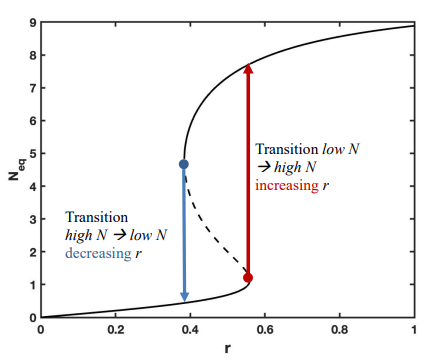
\includegraphics[width = 0.6\textwidth]{figs/bifurcation-diagram-log.png}
\caption{Diagrama de bifurcación. Para el sistema se fija k y se va alterando r. }
\end{figure}

\section{Posibles bifurcaciones en sistemas dinámicos con 1 variable}
Cada bifurcación puede representarse mediante un modelo mínimo (forma normal). Algunas bifurcaciones comunes son:
\begin{enumerate}
\item \textbf{Bifurcación silla-nodo}: Modelada por $dx/dt = r + x^2$. 
\begin{itemize}
\item Para $r < 0$, hay dos puntos de equilibrio, uno estable y otro inestable.
\item Para $r > 0$, no hay puntos de equilibrio.
\item Para $r = 0$, está el punto de bifurcación.
\end{itemize}

\begin{figure}[h]
\centering
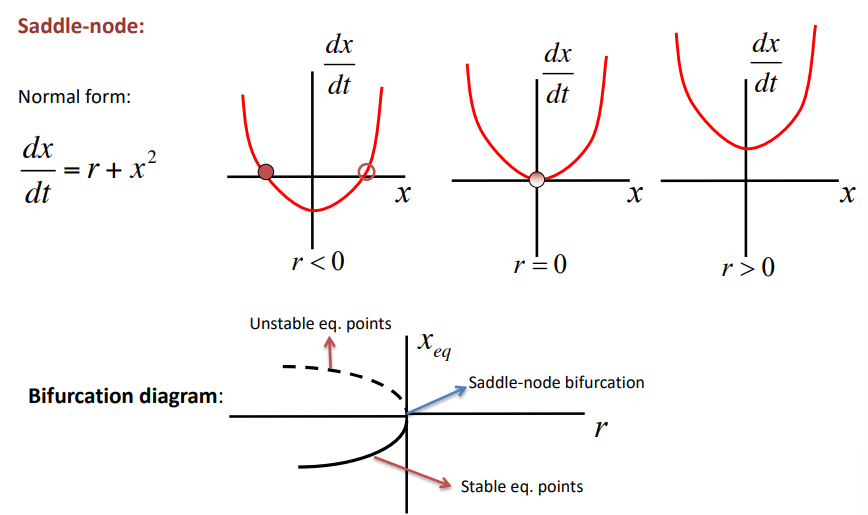
\includegraphics[width = 0.7\textwidth]{figs/saddle-node.png}
\end{figure}

\item \textbf{Bifurcación transcrítica y bifurcación tridente}: Otras bifurcaciones comunes en sistemas de una variable.

\begin{figure}[h]
\centering
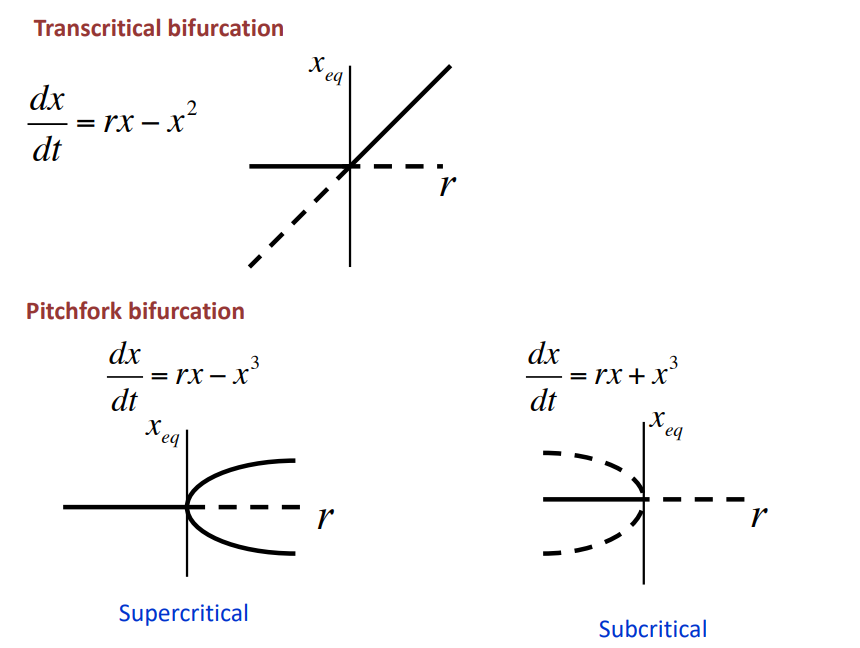
\includegraphics[width = 0.7\textwidth]{figs/bifurcacion-normal.png}
\end{figure}
\end{enumerate}

La estabilidad total (número de estados posibles estables e inestables) antes y después de la bifurcación se conserva. 

\section{Sistemas dinámicos no lineales con dos variables}
\subsection{Modelo de Lotka-Volterra}
El modelo describe la interacción entre presas $N$ y depredadores $P$:
\begin{align*}
\frac{dN}{dt} = N(a - bP) &&
\frac{dP}{dt} = P(cN - d)
\end{align*}

En este modelo tenemos 4 parámetros: crecimiento de presas (a), muerte de presas (b), crecimiento predadores (c), muerte predadores (d). Eso es un modelo complejo, y se puede simplificar cambiando variables "adimensionales". Siendo $u = cN/d$, $v = bP/a$ y $\tau = at$, el sistema se simplifica a:
\begin{align*}
\frac{du}{d\tau} = u(1 - v) &&
\frac{dv}{d\tau} = \alpha v(u - 1).
\end{align*}

Ahora, los puntos de equilibrio solo dependen de $\alpha$ y se componen por dos valores:
$$\begin{pmatrix}
\frac{du}{d\tau}, \frac{dv}{d\tau}
\end{pmatrix} = (0,0) \begin{cases}
(u_{eq}, v_{eq}) = (0,0) \\
(u_{eq}, v_{eq}) = (1,1) 
\end{cases}$$

Para calcular la estabilidad, se pueden pintar por separado las ecuaciones. En el plano de variables u v, se pueden pintar por separado e igualar a cero. Así, se obtienen las nulclinas, y hay dos: la nulclina de u que hace la derivada temporal de u y la nulclina de v, que es la derivada temporal de v. Las nulclinas u y v son rectas en 1. Las dos nulclinas se cortan en el punto de equilibrio, siendo así (1,1).

\begin{figure}[h]
\centering
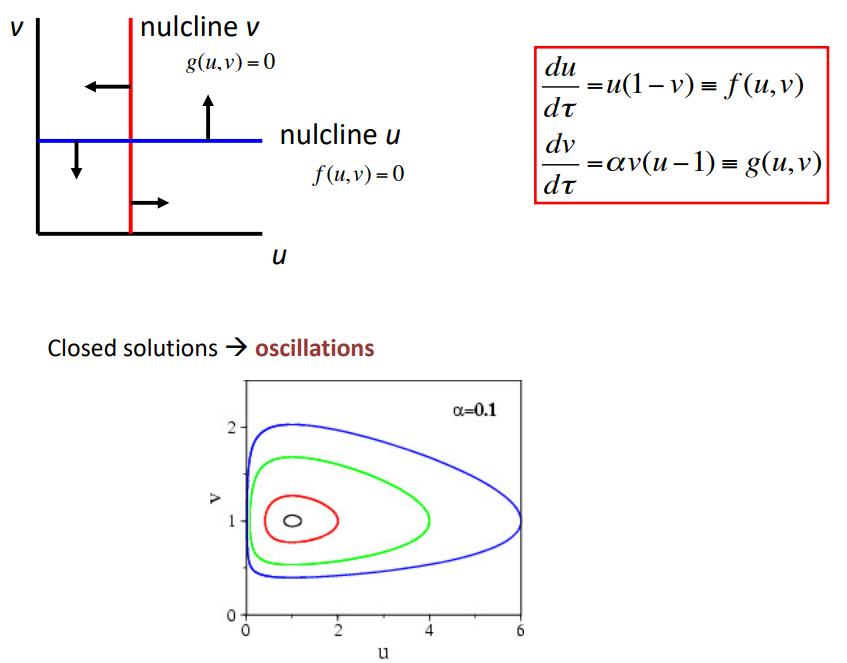
\includegraphics[width = 0.8\textwidth]{figs/nulclinas.png}
\end{figure}

El flujo va en dos direcciones al estar compuestos por un valor de u y otro de v. En una nulclina, el flujo solo va a ser en una dirección, vertical u horizontal. En la nulclina u, el flujo va a ser vertical (en la v) en la dirección según el signo de la derivada; si $u > 1$, el signo de la derivada es positivo y, por tanto, el movimiento es vertical hacia arriba, mientras que si $u < 1$, la derivada es negativa y el movimiento es vertical hacia abajo. 

El punto de equilibrio (1,1) tiene oscilaciones a su alrededor; sigue un comportamiento periódico. Las oscilaciones dependen de la condición inicial. La amplitud y el periodo van cambiando en función de lo lejos que estén del punto de equilibrio. Esto se conoce en física como un \textbf{sistema conservativo}.
Si para un mismo parámetro $\alpha$ cambiamos las condiciones iniciales, las oscilaciones van a cambiar. Las oscilaciones biológicas suelen ser robustas (no cambian de periodo ni de amplitud) con respecto a las condiciones y parámetros iniciales, solo en función de los parámetros (el estado del ambiente/entorno o el tipo de interacciones entre presas y predadores, pero no en función del número de zorros y conejos).

%20/02 - Raúl Guantes
\subsection{Ciclo límite}
Hay un tipo de oscilaciones robustas llamados \textbf{ciclo límite}. Estos ciclos son curvas cerradas en el espacio de variables que son aisladas. En diferentes condiciones iniciales, tanto dentro como fuera de la curva, se converge a ella, ya que es un atractor en forma de oscilación fija. Las condiciones necesarias para que haya un ciclo límite es que haya al menos 2 variables y que sea un sistema no lineal. De hecho, el sistema de Lotka-Volterra de dos variables es un sistema lineal al tener dos variables con exponente 1, por lo que no tiene ciclo límite. Estas condiciones son necesarias, pero no suficientes, ya que también depende de otras condiciones. Intuitivamente, las condiciones son:
\begin{itemize}
\item Tener un punto de equilibrio inestable para que el flujo se vaya fuera.
\item Tener una región cerrada alrededor del punto de equilibrio inestable donde el flujo vaya hacia dentro.
\end{itemize}

\begin{figure}[h]
\centering
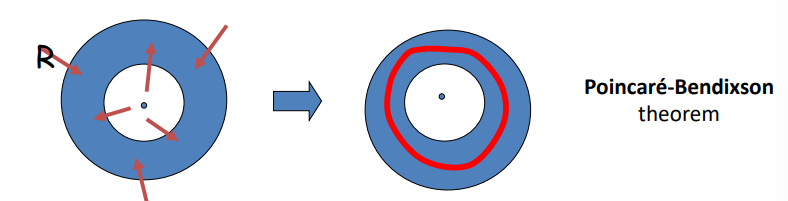
\includegraphics[width = 0.9\textwidth]{figs/ciclo-limite.png}
\end{figure}

\subsection{Generalización del modelo Lotka-Volterra de un ecosistema presa-predador}
El crecimiento de las presas depende de su número y la capacidad de recursos del medio. La ecuación para el número de depredadores es logística. Tiene una casa de crecimiento, pero la capacidad de recursos de los depredadores es el número de presas. 
$$\frac{dx}{dt} = xf(x,y) \rightarrow f(x,y) = r(1 - x/c) - \frac{ky}{x + D}$$
$$\frac{dy}{dt} = yg(x,y) \rightarrow g(x,y) = s(1 - \frac{hy}{x})$$

Se utilizan variables escalares para quedarnos solo con 3 variables, y a continuación se pintan las nulclinas. El punto de corte es el punto de equilibrio, pero éste es inestable. No obstante, hay una curva que indica el ciclo límite. 

\begin{figure}[h]
\centering
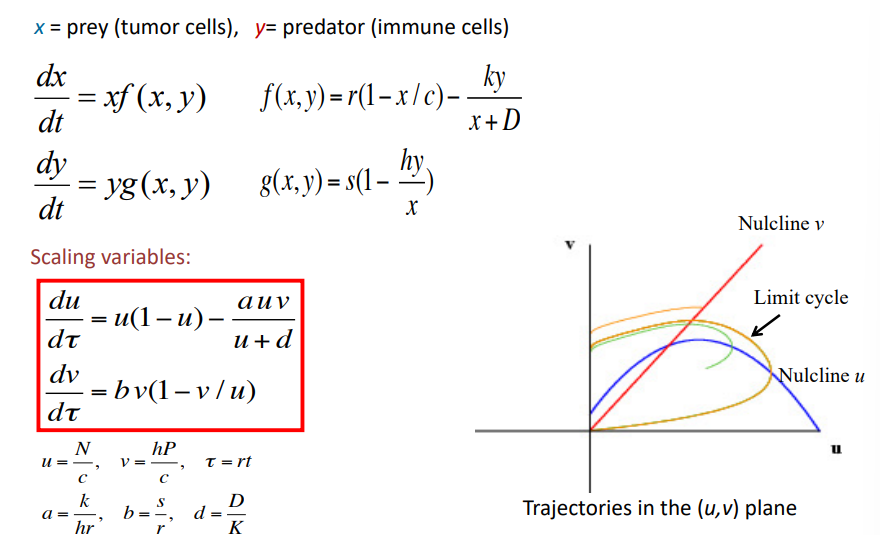
\includegraphics[width = 0.9\textwidth]{figs/ciclo-limite-lv.png}
\end{figure}

Después de un tiempo transitorio, las poblaciones con condiciones iniciales diferentes oscilan con la misma amplitud y el mismo periodo. Esto se debe a que se ha caído en el ciclo límite, y hay oscilaciones robustas. 

Un \textbf{ejemplo} de un sistema presa-predador biológicamente real es con dos poblaciones sintéticas de \textit{E. coli} que interactúen por quorum sensing. Las células predadoras mataban a la presa induciendo la expresión de una proteína letal en las presas. Las presas rescatan a los predadores induciendo la expresión de una proteína antídoto en el predador. 

\subsection{Estabilidad de los puntos de equilibrio en sistemas de 2 (o N) variables por linealización}
Este método se aplica a sistemas dinámicos con dos o más variables, como modelos de presa-depredador, interacciones genéticas, o redes neuronales. Consideremos un sistema con dos variables $u$ y $v$, descrito por las ecuaciones:
\begin{align*}
\frac{du}{dt} = f(u, v) && \frac{dv}{dt} = g(u, v)
\end{align*}

\subsubsection{Puntos de equilibrio}
Los puntos de equilibrio son los valores $(u^{eq}, v^{eq})$ que satisfacen:
\begin{align*}
f(u^{eq}, v^{eq}) = 0 && g(u^{eq}, v^{eq}) = 0
\end{align*}

En estos puntos, el sistema no cambia con el tiempo.

\subsubsection{Linealización alrededor del equilibrio}
Para estudiar la estabilidad de un punto de equilibrio, se introduce una pequeña perturbación $\Delta u$ y $\Delta v$:
\begin{align*}
u = u^{eq} + \Delta u && v = v^{eq} + \Delta v
\end{align*}

Sustituyendo en las ecuaciones dinámicas
$$\frac{du}{dt} = \frac{d(u^{eq} + \Delta u)}{dt} = \frac{du^{eq}}{dt} + \frac{d \Delta u}{dt} = f(u^{eq} + \Delta u, v^{eq} + \Delta v)$$
expandiendo en serie de Taylor alrededor del equilibrio
$$f(u, v) \sim f(u^{eq}, v^{eq}) + \frac{\delta f(u^{eq}, v^{eq})}{\delta u}(u - u^{eq}) + \frac{\delta f(u^{eq}, v^{eq})}{\delta v}(v - v^{eq})$$
, obtenemos:
$$\frac{d \Delta u}{dt} = \frac{\delta f^{eq}}{\delta u} \Delta u + \frac{\delta f^{eq}}{\delta v} \Delta v$$
$$\frac{d \Delta v}{dt} = \frac{\delta g^{eq}}{\delta u} \Delta u + \frac{\delta g^{eq}}{\delta v} \Delta v$$

Estas ecuaciones son lineales y pueden escribirse en forma matricial como:
$$\Delta \vec{x} = \begin{pmatrix}
\Delta x \\ \Delta v
\end{pmatrix} $$

$$\frac{d \Delta \vec{x}}{dt} = \begin{pmatrix}
\frac{d \Delta u}{dt} \\ \frac{d \Delta v}{dt}
\end{pmatrix}$$

La matriz J es una matriz de estabilidad o matriz jacobiana.
$$\vec{J} = \begin{pmatrix}
\frac{\delta f^{eq}}{\delta u} & \frac{\delta f^{eq}}{\delta u} \\
\frac{\delta g^{eq}}{\delta u} & \frac{\delta g^{eq}}{\delta v}
\end{pmatrix}$$
Ahora se debe multiplicar J con delta x.
$$\frac{d \Delta \vec{x}}{dt} = \vec{J} \cdot \Delta \vec{x}$$

$$\begin{pmatrix}
\frac{d \Delta u}{dt} \\ \frac{d \Delta v}{dt}
\end{pmatrix} = \begin{pmatrix}
\frac{\delta f^{eq}}{\delta u} & \frac{\delta f^{eq}}{\delta u} \\
\frac{\delta g^{eq}}{\delta u} & \frac{\delta g^{eq}}{\delta v}
\end{pmatrix} \cdot \begin{pmatrix}
\Delta u \\ \Delta v
\end{pmatrix}$$

Si la matriz J fuese diagonal (todo 0 salvo en la diagonal donde está $\lambda$):
$$\frac{d \Delta y}{dt} = \lambda \Delta y \rightarrow \begin{pmatrix}
\frac{d \Delta y_1}{dt} \\ \frac{d \Delta y_2}{dt}
\end{pmatrix} = \begin{pmatrix}
\lambda_1 & 0 \\ 0 & \lambda_2
\end{pmatrix} \cdot \begin{pmatrix}
\Delta y_1 \\ \Delta y_2
\end{pmatrix}$$
Y esto se puede resolver con:
$$\Delta y_1 (t) = \Delta y_1 (0) e^{\lambda_1 t}$$
$$\Delta y_2 (t) = \Delta y_2 (0) e^{\lambda_2 t}$$

En caso de que J no sea así, puede transformar para que sí sea diagonal.

\subsubsection{Autovalores y estabilidad}
La estabilidad del punto de equilibrio depende de los autovalores $\lambda$ de la matriz jacobiana $\vec{J}$. Los autovalores se calculan resolviendo la ecuación característica:
$$\det (\vec{J} - \lambda \vec{I}) = 0$$
donde $\vec{I}$ es la matriz de identidad. Por tanto, si la matriz tuviese inversa, no se podrían calcular los autovalores.
Para una matriz $2 \times 2$, la ecuación característica es:
$$\lambda^2 - Tr(\vec{J} - \lambda \vec{I}) = 0$$
donde:
\begin{itemize}
\item $Tr(\vec{J}) = J_{11} + J_{22}$ es la traza de $\vec{J}$.
\item $\det \vec{J} = J_{11}J_{22} - J_{12}J_{21}$ es el determinante de $\vec{J}$. 
\end{itemize}

Primero se calculan los puntos de equilibrio, y para cada uno de ellos se calcula la matriz jacobiana. Cada punto de equilibrio tendrá su propio sistema. Después se calculan los autovalores de J con la ecuación característica. Dependiendo de los autovalores, vemos qué tipo de estabilidad tiene el punto de equilibrio. 

Suponemos que tenemos una matriz jacobiana ya calculada. Se debe restar $\lambda$ en la diagonal y se calcula el determinante. Se multiplican los valores de la diagonal y se resta la multiplicación de la otra diagonal. 

$$(J_{11} - \lambda) (J_{22} - \lambda) - J_{12} J_{21} = J_{11} J_{22} - J_{11} \lambda - J_{22} \lambda + \lambda^2 - J_{12} J_{21} = 0$$
$$\lambda^2 - (J_{11} + J_{22}) \lambda + (J_{11} J_{22} - J_{12} J_{21}) = 0$$
$$Tr(J) = J_{11} + J_{22} \equiv Z$$
$$\lambda^2 - Z \lambda + \det J = 0$$ %Mitternachtsformel
$$\lambda_{1,2} = \frac{Z \pm \sqrt{Z^2 - 4\Delta}}{2}$$
De esto salen:
$$\Delta x_1(t) = \Delta x_1(0) \cdot e^{\lambda_1 t}$$
$$\Delta x_2(t) = \Delta x_2(0) \cdot e^{\lambda_2 t}$$
%Saber determinante y traza de las matrices, esto es importante

Si la raíz es positiva, y tenemos autovalores reales, pueden darse varios casos:
\begin{itemize}
\item $\lambda_+ > \lambda_- > 0$: nodo inestable
\item $\lambda_- < \lambda_+ < 0$: nodo estable
\item $\lambda_+ > 0 > \lambda_-$: punto silla, inestable
\end{itemize}

Si la raíz es imaginaria al tener un contenido negativo, se divide la parte real de la imaginaria. 
$$\lambda_{\pm} = Re(\lambda) + iIm(\lambda)$$
$$Re(\lambda_{\pm} = Z/2$$
$$e^{\lambda_{\pm} t} = e^{Re(\lambda) t} e^{i Im(\lambda t)}$$

Volvemos a tener varios casos:
\begin{itemize}
\item Si $Re (\lambda) > 0$: espiral inestable
\item Si $Re(\lambda) < 0$: espiral estable
\item Si $Re(\lambda) = 0$: centro
\end{itemize}

Volviendo al modelo de Lotka-Volterra:
\begin{align*}
\frac{dN}{dt} &= N(a - bP) \rightarrow f(u,v), \
\frac{dP}{dt} &= P(cN - d) \rightarrow g(u, v)
\end{align*}

Calculamos la matriz jacobiana:
$$\vec{J} = \begin{pmatrix}
\frac{\delta f^{eq}}{\delta u} & \frac{\delta f^{eq}}{\delta u} \\
\frac{\delta g^{eq}}{\delta u} & \frac{\delta g^{eq}}{\delta v}
\end{pmatrix}$$

Calculamos las derivadas parciales normales:
$$ \begin{pmatrix}
1 - v & -u \\
\alpha v & \alpha(u - 1)
\end{pmatrix} $$

Y ahora en el punto de equilibrio (1,1):
$$\vec{J} = \begin{pmatrix}
0 & -1 \\ \alpha & 0
\end{pmatrix}$$

Con esto se calculan los autovalores:
$$\lambda^2 + \alpha = 0$$
$$\lambda = \pm \sqrt{- \alpha} = \pm i\sqrt{\alpha}$$
Así, el punto (1,1) es el centro, por lo que tiene oscilaciones.

\subsection{Bifurcaciones de ciclos límite}
La bifurcación Hopf es una espiral estable que se vuelve inestable. Esto ocurre cuando dos autovalores complejos cambian el signo de su parte real. Esto implica que:
\begin{itemize}
\item $\det (\vec{J}) > 0$
\item $Tr(\vec{J}) = 0$
\end{itemize}
para algunos valores de los parámetros.